\documentclass[12pt]{article}
\usepackage{text_style}
\title{Likelihood on the CP-DAG in causal discovery}
\author{IA pour la Science}
\date{6 April 2026}
\begin{document}
\maketitle
\begin{abstract}
For a given dataset of observations maximize the likelihood of the causal graph that generates the reconstruction data.
Estimate the likelihood of the DAG in the linear causal model.
Use Markov equivalence classes of DAGs.
\end{abstract}

\section{Problem statement for graph optimization}
There given~$m$ observations $\mathbf{x}\in\mathbb{R}^n$ %$\bD = \{\mathbf{x}_i\in\mathbb{R}^n\}$
of a random variable~$X$.
The structural causal model is
\begin{equation}
    \hat{\bx} = \bW\mathbf{x} + \boldsymbol{\varepsilon}, \qquad \boldsymbol{\varepsilon} \sim \mathcal{N}(\mathbf{b}, \bSig),
    \label{eq:lin_scm}
\end{equation}
$\bSig = \mathrm{diag}(\sigma_1^2, \dots, \sigma_n^2)$ is the diagonal noise covariance.
Denote by~$f$ the model~\eqref{eq:lin_scm} and its parameters $\bw = (\bW, \mathbf{b})$. %text(vec)
The directed acyclic graph~$G$ defines the structure of the model~$f$, so that for
\[
    \fG \defeq f(\mathbf{x}; \bw, G): \bx \mapsto \hat{\bx}
\]
a model parameter $w_{j} = 0$ if the corresponded element of adjacency matrix~$\bG$ is zero.

The problem is to estimate the most probable DAG structure $p(G\mid X)$ given
%the data $\bD$
the observed variable $X$ and the model $f$:
\begin{equation}
    p(G \mid X, \fG) = p(X \mid \fG) p(G) \to \max_{G},
    \label{eq:bayes_score}
\end{equation}
where $p(G)$ is a prior over DAGs and $p(X \mid \fG)$ is the likelihood of the data given the DAG structure.

The term $p(X \mid \fG)$ is the marginal likelihood of the data given the DAG structure, obtained by integrating out the parameters $\bw$:
\begin{equation}
    p(X \mid \fG) = \int p(X \mid \bw, \fG) p(\bw \mid \fG) d\bw
    \label{eq:marginal_likelihood}
\end{equation}
where $p(\bw \mid \fG)$ is the prior over the parameters given the DAG structure.

Assume the distribution of the model parameters $p(\bw \mid \fG) = \cN(\bmu, \bA)$ and
with the assumption from~\eqref{eq:lin_scm} rewrite the integrated part from likelihood term~\eqref{eq:marginal_likelihood} as:
\begin{equation}
    p(\bw \mid \bx, \fG) = \frac{1}{2} \sum_i (\bx_i - \hat{\bx}_i)\T \bSig^{-1} (\bx_i - \hat{\bx}_i)
    + \frac{1}{2} (\bw - \bmu)\T \bA^{-1} (\bw - \bmu).
    \label{eq:likelihood_prior}
\end{equation}
The parameters of the prior~$\bmu, \bA$ and covariance matrix~$\bSig$ is estimated during the optimization algorithm. %FIXIT~\ref{alg:one}.
The covariance matrix~$\bA$ plays its role in the sampling of the nodes of the graph~$G$.

\begin{figure}[ht]
    \centering
    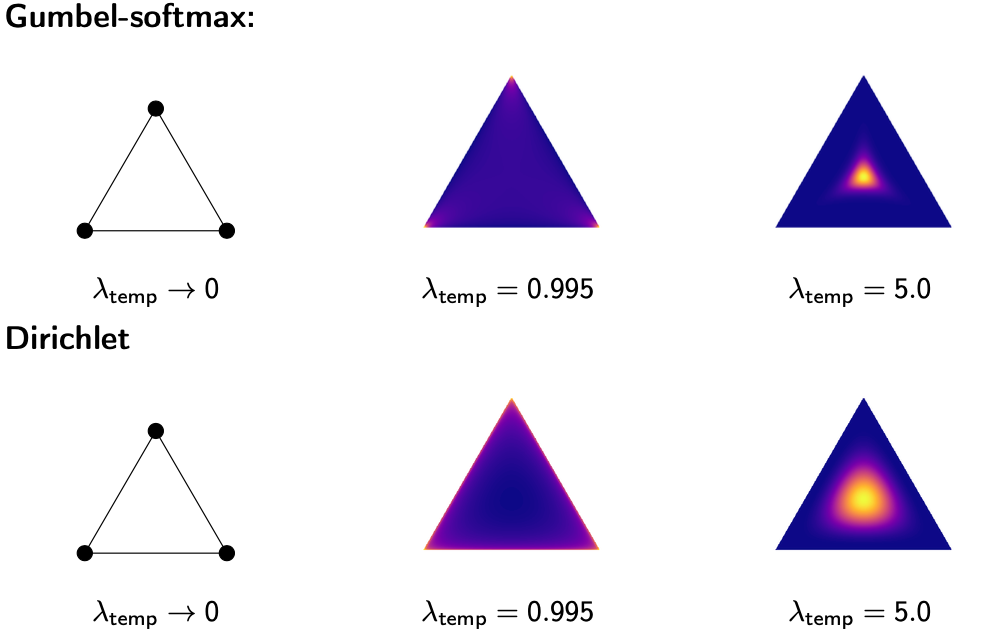
\includegraphics[width=0.8\textwidth]{fig_dir_gs}
    \caption{The Dirichlet and Gumbel-Softmax distributions for different values of the temperature $\tau$. As $\tau \to 0$ the density concentrates near the vertices of the simplex (one-hot vectors).
As $\tau=\lambda_\text{temp}$ increases, it becomes smoother.}
    \label{fig:gumbel_softmax}
\end{figure}

Assume several independent hypotheses of the graph~$G$ distribution over the set of DAGs:
\begin{enumerate}[1)]
    \item $p(G) = \text{const}$, the uniform prior,
    \item $p(G) \propto e^{-\gamma |G|}$, a sparsity-inducing prior,
    \item $p(G) \propto e^{-\gamma h(G)}$, where $h(G)$ is a smooth acyclicity constraint,% (NOTEARS),
    \item $p(G)$ is a Dirichlet distribution
    \[ \mathrm{Dir}(\mathbf{y} \mid \boldsymbol{\pi}) = \frac{\Gamma \left(\sum_{i=1}^k \pi_i\right)}
    {\prod_{i=1}^k \Gamma(\pi_i)}\prod_{i=1}^k y_i^{\pi_i - 1},
    \]
    \item $p(G) \propto \text{GS}(\boldsymbol{\pi},\tau)$, the concrete (relaxed) Gumbel-Softmax distribution
    \[
    p(\mathbf{y} \mid \boldsymbol{\pi}, \tau) = \Gamma(k),\tau^{k-1}
    \left( \sum_{i=1}^{k} \frac{\pi_i}{y_i^{\tau}} \right)^{-k}\prod_{i=1}^{k} \frac{\pi_i}{y_i^{\tau+1}}.
    \]
\end{enumerate}
The last two distributions have the parameters $\boldsymbol{\pi} = (\pi_1, \dots, \pi_i > 0, \dots, \pi_k)$, are the unnormalized log-probabilities of edges of the simplex
\[
\mathbf{y} \in \Delta^{k-1} = \left\{ \mathbf{y} \in \mathbb{R}^k : y_i > 0, \sum_{i=1}^{k} y_i = 1 \right\}
\]
and $\tau$ is the temperature controlling the smoothness of the distribution.
Figure~\ref{fig:gumbel_softmax} illustrates the effect of~$\tau$.
The Gamma function $\Gamma(k)$ has $k$ categories, edges of the graph $G$.
This is a continuous distribution on the simplex so the change $d\by$ is computable.

State the optimization problem
\begin{equation}
    \loss (\bw; \bx, \fG)  = \loss_\bx + \loss_\bw + \loss_G \to \min\limits_{G\in\mathcal{G}}
    \label{eq:optimization_problem}
\end{equation}
using \eqref{eq:likelihood_prior} and the listed above prior over DAGs.
The problem~\eqref{eq:optimization_problem} includes the bayesian hyperparameters:
\begin{itemize}
    \item[] the diagonal covariance matrix $\bSig$ controls the noise level in the data,
    \item[] the mean and covariance $\bmu, \bA$ control the prior over parameters $\bw$,
    \item[] $\boldsymbol{\pi}$ controls the unnormalized log-probabilities of edges of the graph,
    \item[] $\gamma$ controls the sparsity of the graph,
    \item[] $\tau$ controls the smoothness of the distribution over graphs.
\end{itemize}
The plate notation of the probabilistic model is shown in Figure~\ref{fig:plate}.

\begin{figure}[ht]
    \centering
    \begin{tikzpicture}
        % Nodes (left side)
        \node[latent] (s) {$\boldsymbol{\pi, \tau}$};
        \node[latent, right=of s] (Gamma) {$G$};
        \node[latent, below=of s] (A) {$\bA,\bmu$};
        \node[latent, right=of A] (W) {$\bw$};
        % Nodes inside plate (gray shaded)
        \node[latent, fill=gray!30, right=3cm of Gamma] (xi) {$\bx_i$};
        \node[latent, fill=gray!30, below=of xi] (yi) {$\hat\bx_i$};
        % Edges
        \edge {s} {Gamma};
        \edge {Gamma} {W};
        \edge {A} {W};
        \edge {Gamma} {yi};
        \edge {W} {yi};
        \edge {xi} {yi};
        % Plate
        \plate {plate1} {(xi)(yi)} {$i = 1, \dots, m$};
        \end{tikzpicture}
    \caption{The plate notation of the causal structure model.
    The nodes $\bx_i$ and $\hat\bx_i$ are observed and reconstructed variables.
    The parameters $\boldsymbol{\pi}, \tau$ control the distribution over DAGs.
    The hyperparameters $\bA, \bmu$ control the prior over the model parameters $\bw$.}
    \label{fig:plate}
\end{figure}

\section{MCMC sampling of the DAG structure}
The generic sampling procedure for the DAG structure includes the estimation of the
parameters and hyperparameter of the structure causal model.
\begin{enumerate}
    \item Sample the DAG structure $G$ from the prior distribution $p(G)$.
    \item Check its admissibility  and the acyclicity constraint $h(G) = 0$.
    \item Construct the corresponding structure causal model $f_G$.
    \item Use the prior parameters $\bA, \bmu$.
    \item Optimize the model parameters $\bw$ by minimizing the loss function $\loss_x$.
    \item Sample subsets of the data $\bx$ to estimate new hyperparameters~$\bSig, \bA, \bmu$.
    \item Compute the likelihood $\loss =\loss_\bx + \loss_\bw + \loss_G$.
    \item Correct the distribution of the DAG structure $G$ (by accepting or rejecting it based on the likelihood $\loss$).
    \item Repeat the procedure until convergence of loss $\loss$.
\end{enumerate}

\subsection*{Genetic sampling algorithm}
The Genetic algorithm as a simple heuristical replacement of the MCMC sampling.
Introduce the indicator vector $\ba \mapsto G$ that restores an admissible graph structure.
This vector is a vertex in the binary cube $\ba \in \{0, 1\}^d$,
where $d$ is the number of possible edges in the graph.
For a graph with $n$ nodes $d \leq \frac{1}{2}n(n-1)$.
The genetic algorithm includes the following steps:
\begin{enumerate}
    \item There is a are set of binary vectors
    \[
      \{\ba_1, \dots, \ba_P \}, \ba\in\{0,1\}^d.
    \]
    \item Get two uniformly random vectors $\ba_p, \ba_q$, their indexes $p, q \in \{1,\dots,P\}$.
    \item Choose a random number $v \in \{1, \dots, n-1\}$.
    \item Split both vectors and change their parts:
    \[
        [a_{p,1}, \dots, a_{p,v} \mid a_{q,v+1}, \dots, a_{q,n}] \to \ba^\prime_p,
    \]
    \[
        [a_{q,1}, \dots, a_{q,v} \mid a_{p,v+1}, \dots, a_{p,n}] \to \ba^\prime_q.
    \]
    \item Choose random numbers $r_1, \dots, r_Q \in \{1, \dots, n\}$.
    \item Invert positions $r_1, \dots, r_Q$ of the vectors $\ba^\prime_p,\ba^\prime_q$.
    \item Repeat $P/2$ times the items 2--6.
    \item Evaluate the obtained models, compute the loss $\loss$.
    \item Keep the best $P$ vectors $\ba$ with the lowest loss $\loss$ and discard the rest.
\end{enumerate}
Repeat the algorithm until convergence of the loss $\loss$ or a fixed number of iterations.
Here $P, Q$ are the heuristic parameters of the algorithm.

\begin{figure}[ht]
    \centering
    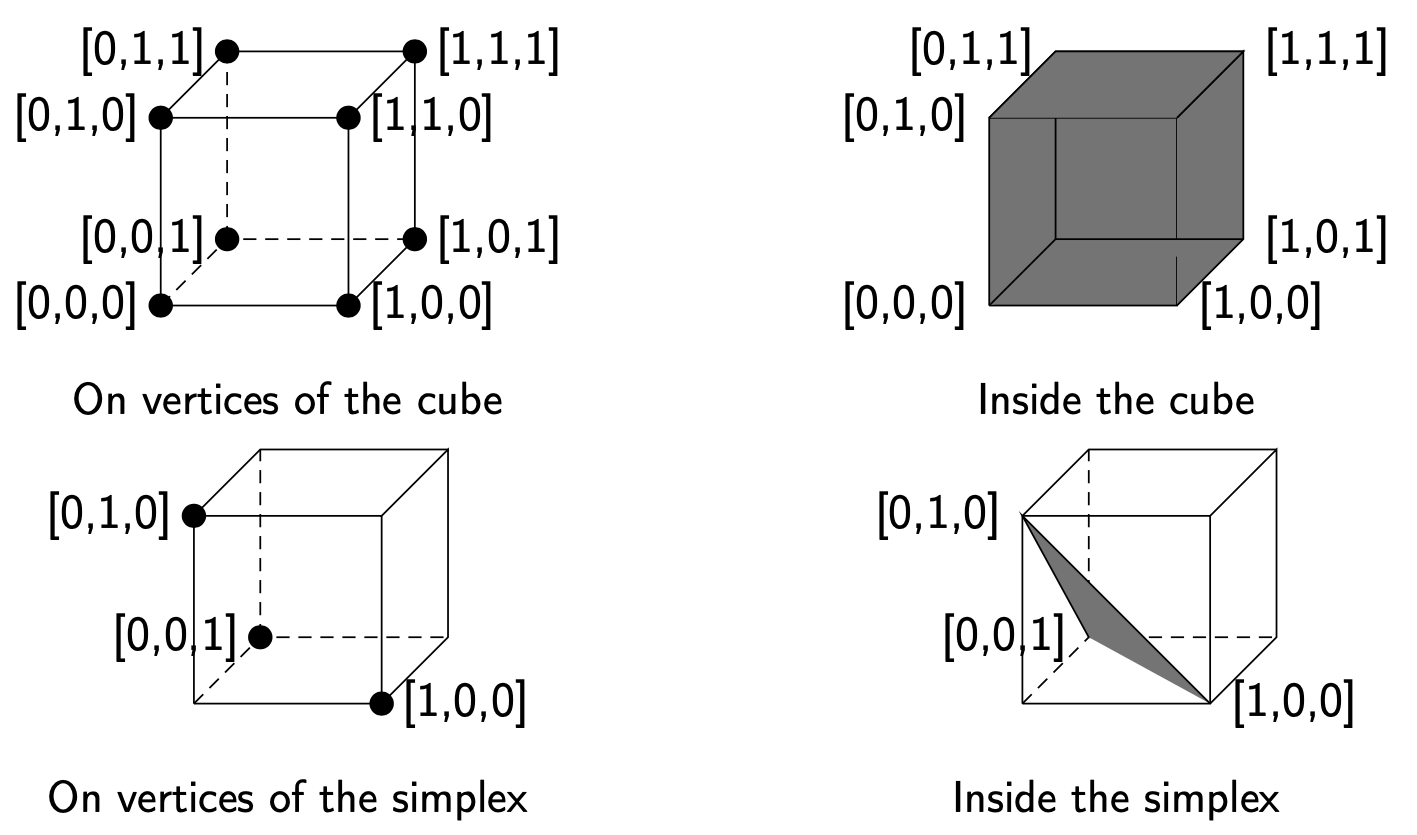
\includegraphics[width=0.8\textwidth]{fig_cube}
    \caption{ The restrictions to the structure parameters. Examples for some structure parameter.}
    \label{fig:cube}
\end{figure}

\subsection*{MCMC sampling algorithm}
To sample graphs~$\bw_0 = \{\bw \mid \bw \sim p(\bw|\boldsymbol{\pi})\}$ that deliver models with the best likelihood,
use Metropolis-Hastings sampling version of the Markov Chain Monte Carlo sampling algorithm.
The basic idea of the algorithm is to generate a sample such that the sample  forms a Markov chain.
Each element $\bw_{t+1}$ of the sample depends on the previous element $\bw_t$ of the sample  only.
Denote by $Q(\bw \mid \bw^\prime)$ an auxiliary distribution $Q(\bw\mid \bw^\prime)$.
Choose an initial element $\bw_0$ and assign $\bW_0 = \{\bw_0\}$.
Then let an element $\bw_t$ be chosen according  to the distribution $Q(\bw^\prime\mid\bw_t)$.
The next element $\bw^\prime$ is generated randomly.
Then the algorithm computes the acceptance ratio $a$:
\[
    a = \min\limits_{\bw^\prime\in\mathbb{R}^n}\left(
    \frac{p(D\mid\bw^{\prime}, B_0)\quad Q(\bw_t\mid\bw^\prime)}
    {p(D\mid\bw_t, B_0)\quad Q(\bw^\prime\mid \bw_t)}, 1\right).
\]

The algorithm accepts the candidate $\bw^\prime$ with the probability $a$,
\[
    \bw_{t+1} = \bw^\prime, \qquad, W_0 := W_0 \cup \bw^\prime.
\]
Otherwise, the algorithm rejects the candidate and puts $\bw_{t+1} = \bw_t$,
\[
\bw_{t+1} =
\begin{cases}
\bw^\prime, \quad\text{with the probability}\quad a,
\bw_t, \quad\text{with the probability} (1-a).
\end{cases}
\]
Let the auxiliary distribution $Q(\bw \mid \bw^\prime)$ be normal:
\[
    Q(\bw \mid \bw^\prime) = Q(\bw^\prime \mid \bw) = \frac{1}{(2\pi\alpha^{-1})^{n/2}} \exp\left(-\frac{\alpha}{2}(\bw - \bw^\prime)\T (\bw - \bw^\prime)\right).
\]
That is, the function $Q(\bw \mid \bw^\prime)$ is symmetric and
the acceptance ratio $a$ simplifies to
\[
    a = \min\limits_{\bw^\prime\in\mathbb{R}^n}\left(
    \frac{p(D\mid\bw^{\prime}, B_0)}{p(D\mid\bw_t, B_0)}, 1\right).
\]
The initial element $\bw_0$ is chosen randomly from the distribution $p(\bw \mid \boldsymbol{\pi})$.

\subsection*{Direct optimization of the DAG structure}
The continuous optimization of the DAG structure requires two-step procedure:
\begin{enumerate}
    \item Given some parameters~$\bw$ construct a linear approximation of the model $f$.
    \item Make a gradient step to optimize the graph structure
    \[
        \nabla_\ba = \frac{\partial \loss}{\partial \ba} = \frac{\partial \loss}{\partial {\bx}} \cdot \frac{\partial {\bx}}{\partial \ba}.
    \]
    \item Update the structure parameters $\ba$.
    \item Make several steps of the optimization of the model parameters $\bw$,
    \[
        \nabla_\bw = \frac{\partial \loss}{\partial \bw} = \frac{\partial \loss}{\partial {\bx}} \cdot \frac{\partial {\bx}}{\partial \bw}.
    \]
\end{enumerate}
For a linear mode this algorithm is equivalent to the quadratic optimization problem
\[
    \min_\ba\loss(\bw; \bx, \fG) = \lambda \ba\T \mathbf{Q} \ba + (1-\lambda) \mathbf{x}\T \ba.
\]
\end{document}